\documentclass[12pt,a4paper]{article}

\usepackage[utf8]{inputenc}
\usepackage[greek,english]{babel}
\usepackage{float}
\usepackage[export]{adjustbox}
\usepackage{sans} \usepackage{kerkis} 
%\usepackage{sans}
%\usepackage[LGRgreek]{mathastext}   
\usepackage{graphicx}
%\usepackage{enumerate}
\usepackage{enumitem}  
\usepackage{amsmath}
\usepackage{hyperref,xcolor} 
\usepackage{subcaption}

\hypersetup{
    colorlinks,
    linkcolor={black!50!black},
    citecolor={blue!50!black}, urlcolor={cyan!80!black},
}

\newcommand{\en}{\selectlanguage{english}} 
\newcommand{\tl}{\textlatin} 
\newcommand{\gr}{\selectlanguage{greek}}   
\newcommand{\code}[1]{\texttt{#1}}         
%\newcommand{\tsuper}{\textsuperscript} \newcommand{\tsub}{\textsubscript}

 \renewcommand{\thesection}{\arabic{section}.} 
% \renewcommand{\thesubsection}{\arabic{subsection}.}


\gr \title{{\bf 
\includegraphics[scale=1.0]{images/up_landscape.jpeg} \\ ΤΜΗΜΑ ΜΗΧΑΝΙΚΩΝ ΗΛΕΚΤΡΟΝΙΚΩΝ ΥΠΟΛΟΓΙΣΤΩΝ ΚΑΙ ΠΛΗΡΟΦΟΡΙΚΗΣ  \\ \vspace{3cm}Αναφορά Εργαστηριακής Άσκησης Μέρος Β' \\ Υπολογιστική Νοημοσύνη}}
\author{Κωνσταντίνος Τσάκωνας \\ Α.Μ.: 1059666}
\date{Ακαδημαϊκό έτος 2020-21\\ Εαρινό Εξάμηνο}

\begin{document}

    \gr \maketitle \newpage

    \tableofcontents  \newpage

    \section*{\tl{Repository} \gr Κώδικα}
        Για την ανάπτυξη της άσκσης χρησιμοποιήθηκε η γλώσσα \tl{Python} με τις βιβλιοθήκες \tl{Tensorflow, numpy, pandas, deap} και \tl{matplotlib}. Παρακάτω υπάρχει το \tl{repository} του κώδικα στο \tl{github} \\
        \underline{\tl{\textbf{\href{https://github.com/iamtsac/computational-intelligence-part-b}{github link}}}}

        \section*{Β1. Σχεδιασμός ΓΑ}
            \begin{enumerate}
                \item Τα άτομα του αρχικού πληθυσμού θα αναπαραστηθούν ως
                    δυαδικές συμβολοσειρές. Ο λόγος που θα ακολουθηθεί αυτή η
                    κωδικοποίηση προέρχεται από το σκεπτικό ότι, αυτό που
                    θέλουμε να κάνουμε είναι να μειώσουμε το είσοδους από τα 784
                    \tl{pixels}, δηλαδή να μηδενισούμε πολλες από αυτές.
                    Δημιουργώντας λοιπόν άτομα του πληθυσμού ως πίνακες 784
                    \tl{pixels} που περιέχουν δυαδικά στοιχεία, μπορούμε με ένα
                    πολλαπλασιασμό \tl{element-wise} να κρατήσουμε τις εισόδους που
                    θέλουμε.
                \item Ο αρχικός πληθυσμός θα είναι \tl{N} τυχαίοι πίνακες
                    28\tl{x}28 και οι τιμές που θα περιέχουν θα είναι 0 και 1.
                \item Η συνάρτηση καταλληλότητας που επιλέχθηκε είναι οι εξής:
                    \begin{itemize}
                        
                        \item κάθε φορά που θα γίνεται έλεγχος στο νευρωνικό
                            σύμφωνα με τις εισόδους που προκύπτουν από κάθε
                            άτομο του πληθυσμού θα κάνουμε ταξινόμιση των πρώτων
                            $10.000$ εικόνων και θα συγκρίνουμε την ταξινόμιση
                            αυτή με βάση τα \tl{labels} για να δούμε πόσο
                            ακριβής είναι. Το αποτελέσμα που θα προκύπτει από
                            αυτο θα είναι μια τιμή μεταξύ του διαστήματος
                            $[0,1]$
                            και στόχος του γενετικού αλγοριθμού θα είναι να
                            πλησιάσει όσο το δυνατό πιό κοντά στο $1$.
                        \item Επίσης θα επιβάλεται μία ποινή σε άτομα του
                            πληθυσμού που έχουν μεγάλο αριθμό εισόδων,
                            συγκεκριμένα άτομα που έχουν περισσότερες από $392$
                            εισόδους θα αφαιρείται μία τιμή η οποία θα είναι
                            ανάλογη με το ποσοστό που δεν ταξινομήθηκε σώστα επί
                            το πλήθος των παραπάνω εισόδων που έχει σε σχέση με
                            αυτές που έχουμε θέσει ως επιθυμητό άνω όριο.

                    \end{itemize}
                    Ο λόγος που επιλέχθηκε η μεγιστοποίηση του ποσοστού
                    ταξινόμισης έχει να κάνει με το γεγονός ότι κατά την δημιουργία και την
                    εκπαίδευση του μοντέλου στην προηγούμενη εργαστηριακή άσκηση
                    σε πάρα πόλυ μικρές τιμές του \tl{loss} η ταξινόμιση δεν
                    ήταν πάντα σωστή και δεν συμβάδιζε με το \tl{accuracy} του
                    μοντέλου. Ακόμα ο λόγος που εφαρμόζουμε ποίνη σε άτομα που
                    έχουν περισσότερες από $392$ εισόδους είναι γιατί θα έχουμε
                    μία μείωσει $50\%$ αλλά για λιγότερες εισόδους από αυτές θα
                    χάνουμε χαρακτηριστικά που χρειαζόμαστε αφού το σχήμα των
                    ψηφιών στις είκονες συνεχώς μεταβάλεται, με αποτέλεσμα να
                    μην έχουμε καλή ταξινόμιση.

                \item Γενετικοί Τελεστές:
                    \begin{enumerate}
                        \item Επιλογή:
                        \begin{itemize}
                                \item Ρουλέτα βάσει κόστους: Με αυτή την μέθοδο από Ν 
                                    άτομα επιλέγουμε με βάση μία 
                                    πιθανότητα \tl{$p_i$} τα άτομα τα οποία θα γίνει η δισταύρωση. Η 
                                    πιθανότητα υπολογίζεται ως εξής: 
                                    $$ p_i = \frac{f_i}{\sum_{i=1}^{N}f_i}$$
                                     όπου, \\ $f_i$: το \tl{fitness} του \tl{i}-οστού ατόμου,\\
                                    Ν: το μέγεθος του πληθυσμού.
                                    \\ Κατα αυτό τον τρόπο τα άτομα με το μεγαλύτερο \tl{fitness} 
                                    έχουν μεγαλύτερη πιθανότητα να επιλεγούν, δηλαδή βαρένουν περισσότερο.
                                    \item  Ρουλέτα βάσει κατάταξης: Με την μέθοδο αυτή τα 
                                        άτομα κατατάσονται με
                                        σύμφωνα με την καταλληλότητα σε αύξουσα σειρά. Στο 
                                        άτομα με τη μικρότερη 
                                        καταλληλότητα ανατείθεται κατάταξη 1, στο αμέσως επόμενο 2
                                        και η διαδικασία συνεχίζεται μεχρί το
                                        καταλληλότερο άτομα να έχει κατάταξη Ν, όπου 
                                        Ν το μέγεθος του πληθυσμού.
                                        Το μέγεθος που πιάνει το άτομα πάνω στη ρουλέτα σε 
                                        τοις εκατό προκύπτει από:
                                        $$\frac{r_i}{\sum_{i=1}^{N}r_i}\times100$$
                                        όπου,
                                        \\ $r_i$: η κατάταξη του \tl{i}-οστού ατόμου,\\ 
                                        Ν: το μέγεθος του πληθυσμού.
                                        \\ Σύμφωνα με το παραπάνω τα άτομα βαρύνουν με 
                                        τον ίδιο τρόπο ανεξαρτήτως της
                                        μεγάλης απόκλισης που μπορεί να έχει η συνάρτηση 
                                        καταλληλότητας τους.
                                        \\
                                    \item Τουρνουά: Με την μέθοδο αυτή 
                                        δημιουργούμε ένα τουρνουά μεγέθους Κ. Σε κάθε 
                                        τουρνούα διαλέγουμε τυχαία Κ άτομα, από αυτά επιλέγεται αυτό 
                                        με το καλύτερο 
                                        \tl{fitness}. %Τα άτομα που παιρνάνε στην
                                        %επόμενη γενιά δεν αφαιρούνται από τον πληθυσμό με αποτέλεσμα να μπορούν να 
                                        %επιλεγούν ξανά.
                                        \\
                        \end{itemize}
                        Από αυτές αυτή που επιλέχθηκε για τον αλγόριθμο μας σύμφωνα με το πρόβλημα 
                        που έχουμε να 
                            επιλύσουμε είναι η μέθοδος του Τουρνουά. Ο λόγος που επιλέχθηκε
                            βασίζεται στο γεγονός ότι
                            τα άτομα που θα επιλεγούν για να διασταυρωθούν θα έχουν μεγαλύτερες
                            διαφοροποιήσεις μεταξύ τους, διότι επιλέγονται Κ άτομα τυχαία. 
                            Στις υπόλοιπες μεθόδους 
                            οι επιλογή γίνεται με βάση κάποια πιθανότητα από τον αρχικό πληθυσμό με 
                            αποτέλεσμα τα άτομα
                            με καλύτερη καταλληλότητα να είναι πιο πιθανό να επιλεγούν. Άρα με την 
                            χρήση του τουρνουά και
                            την ποικολομορφοία που προσφέρει στη διασταύρωση μπορεί να προκύψει κάποιο 
                            άτομο με πολύ
                            καλύτερο \tl{fitness} από το καλύτερο άτομο της προηγούμενης γενιάς 
                            με αποτέλεσμα ο αλγόριθμος
                            να συγκλείνει πιο γρήγορα.
                    \item Διασταύρωση: 

                        \begin{itemize}
                                \item Διασταύρωση μονού σημείου: Κατά την
                                    διασταύρωση μονού σημείου δημιουργούνται
                                    ζευγάρια ατόμων από αυτά που επιλέχθηκαν και
                                    επιλέγεται τυχαία ένας ακέραιος αριθμός Ν.
                                    Τα άτομα είναι μήκους Μ και ισχύει ότι 
                                    $0\leqΝ\leqΜ-1$. Το Ν είναι το σημείο που θα
                                    γίνει η διασταύρωση των ατόμων, δηλαδή θα
                                    γίνει ανταλλαγή των δυαδικών ψηφίων Ν μέχρι
                                    $Μ-1$.
                                \item Διασταύρωση διπλού σημείου: Η μέθοδος
                                    είναι ίδια με την παραπάνω με την διαφορά
                                    οτί επιλέγονται δύο ακεραίοι αντί ενός και η
                                    διασταύρωση θα γίνει μεταξύ των δυαδικών
                                    ψηφίων που περιέχονται εντός των οριών που
                                    θέτουν οι ακεραίοι που επιλέχθηκαν.
                                \item Ομοιόμορφη διασταύρωση: Για αυτού του
                                    τύπου την διασταύρωση δημιουργείται μια
                                    φόρμα από δυαδικά ψηφία μήκους ίδιου με του
                                    ατόμου. Στα σημεία που η φόρμα έχει τον
                                    ψηφίο 1 το πρώτο παιδί παίρνει το αντίστοιχο
                                    ψηφίο του δεύτερου γονέα, ένω το δεύτερο παιδί του
                                    πρώτου γονέα. Όταν το ψηφίο της φόρμας είναι
                                    0 το πρώτο παιδί παίρνει το αντίστοιχο ψηφιό
                                    το πρώτου γονέα ενώ το δεύτερο παιδί του
                                    δεύτερου γονέα.\\
                        \end{itemize}
                         Στον αλγόριθμο μας επιλέξαμε διασταύρωση διπλού σημείο.
                         Εστιάζοντας στο πρόβλημα που έχουμε, πρέπει να
                         αφαιρέσουμε \tl{pixels} από μία εικόνα αλλά ταυτοχρόνως
                         να μην αφαιρέσουμε σημαντική πληροφορία για τον
                         νευρωνικό μας. Αν χρησιμοποιούσαμε την διασταύρωση
                         μονού σημείου ή την ομοιόμορφη οι απόγονοι κατά το
                         πέρας των γενεών θα περιορίζονταν, δηλαδή θα αφαιρούσαν
                         \tl{pixels} από κοντινές περιοχές και αυτό θα μπορούσε
                         να οδηγήσει σε πολύ χαμηλής ποιότητας λύση αφού αν
                         παρατηρήσουμε τις εικόνες που έχουμε στο σύνολο
                         δεδομένων μας θα δούμε ότι μας ενδιαφέρει κυρίως είναι
                         να αφαιρέσουμε το περίγραμμα και να κρατήσουμε τα
                         κεντρικά \tl{pixels} διότι αυτά είναι που απεικονίζουν
                         τον αριθμό που θέλουμε να ταξινομηθεί.\\

                     \item  Μετάλλαξη:

                        
                    \end{enumerate}

            \end{enumerate}

            \section*{Β3. Αξιολόγηση και επίδραση παραμέτρων}
                \begin{enumerate}


                    \item Πίνακς αποτελεσμάτων \\
                     \begin{tabular}{|p{2em}| p{7em} | p{7em} | p{8em} | p{6.5em} | p{6em} | }
                        \hline
                        \textbf{Α/Α} & \textbf{ΜΕΓΕΘΟΣ ΠΛΗΘΥΣΜΟΥ} &
                        \textbf{ΠΙΘΑΝΟΤΗΤΑ
                            ΔΙΑΣΤΑΥΡΩΣΗΣ} & \textbf{ΠΙΘΑΝΟΤΗΤΑ
                        ΜΕΤΑΛΛΑΞΗΣ} & \textbf{ΜΕΣΗ ΤΙΜΗ ΒΕΛΤΙΣΤΟΥ} & \textbf{ΜΕΣΟΣ
                    ΑΡΙΘΜΟΣ ΓΕΝΕΩΝ}\\
                        \hline
                        1  & 20  & 0.6 & 0.00 & 0.369 & 6  \\
                        \hline
                        2  & 20  & 0.6 & 0.01 & 0.369 & 6  \\
                        \hline
                        3  & 20  & 0.6 & 0.10 & 0.495 & 15 \\
                        \hline
                        4  & 20  & 0.9 & 0.01 & 0.384 & 5.5 \\
                        \hline
                        5  & 20  & 0.1 & 0.01 & 0.404 & 9 \\
                        \hline
                        6  & 200 & 0.6 & 0.00 & 0.739 & 25 \\
                        \hline
                        7  & 200 & 0.6 & 0.01 & 0.725 & 30 \\
                        \hline
                        8  & 200 & 0.6 & 0.10 & 0.810 & 32.5 \\
                        \hline
                        9  & 200 & 0.9 & 0.01 & 0.790 & 21 \\
                        \hline
                        10 & 200 & 0.1 & 0.01 & 0.588 & 19.5 \\
                        \hline

                \end{tabular}

            \item Καμπύλες εξέλιξης:
                \newpage
                \begin{figure}[H]
                     \centering
                     \begin{subfigure}[h]{0.7\textwidth}
                         \centering
                         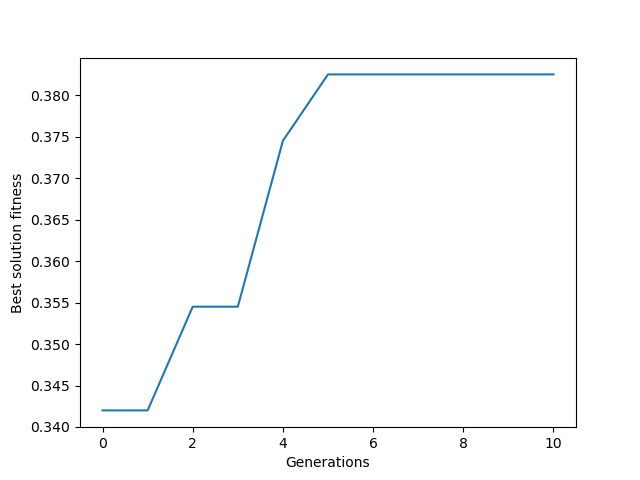
\includegraphics[width=\textwidth]{images/1.png}
                         \caption*{Περίπτωση: 20, 0.6 ,0.00}
                     \end{subfigure}
                     \hfill
                     \begin{subfigure}[h]{0.7\textwidth}
                         \centering
                         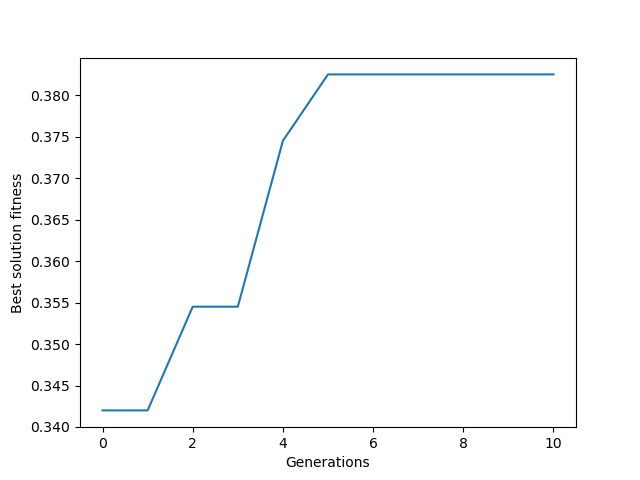
\includegraphics[width=\textwidth]{images/2.png}
                         \caption*{Περίπτωση: 20, 0.6 ,0.01}
                     \end{subfigure}
                     \hfill
                     \begin{subfigure}[h]{0.7\textwidth}
                         \centering
                         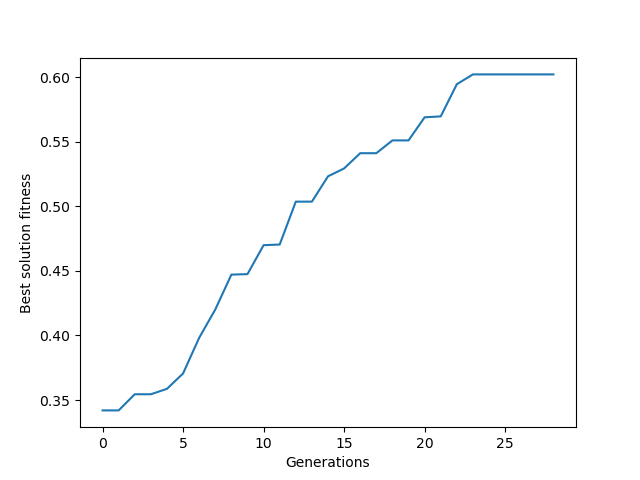
\includegraphics[width=\textwidth]{images/3.png}
                         \caption*{Περίπτωση: 20, 0.6 ,0.10}
                     \end{subfigure}
                 \end{figure}
                 \begin{figure}[H]
                     \centering
                     \begin{subfigure}[h]{0.7\textwidth}
                         \centering
                         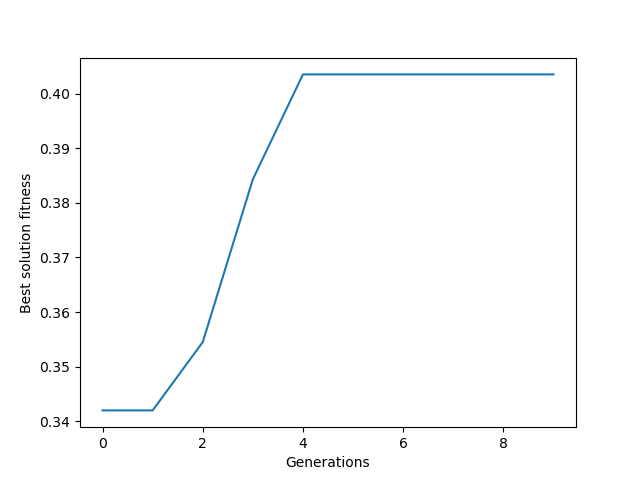
\includegraphics[width=\textwidth]{images/4.png}
                         \caption*{Περίπτωση: 20, 0.9 ,0.01}
                     \end{subfigure}
                     \begin{subfigure}[h]{0.7\textwidth}
                         \centering
                         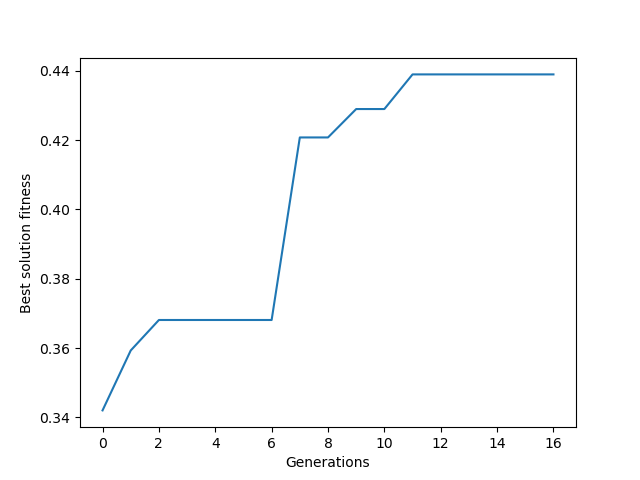
\includegraphics[width=\textwidth]{images/5.png}
                         \caption*{Περίπτωση: 20, 0.1 ,0.01}
                     \end{subfigure}
                     \begin{subfigure}[H]{0.7\textwidth}
                         \centering
                         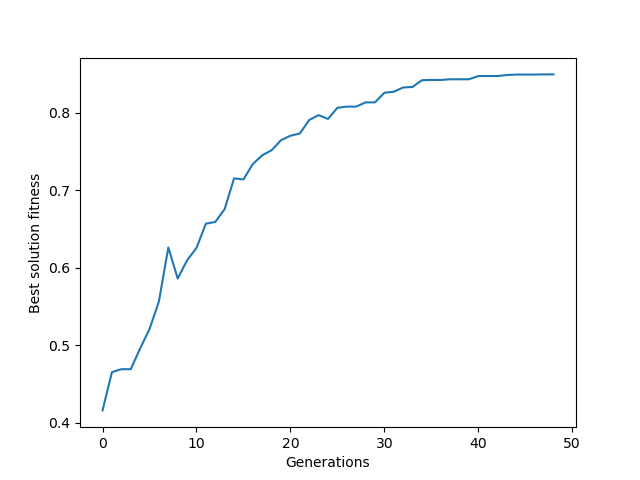
\includegraphics[width=\textwidth]{images/6.png}
                         \caption*{Περίπτωση: 200, 0.6 ,0.00}
                     \end{subfigure}
                 \end{figure}
                 \begin{figure}[H]
                     \centering
                     \begin{subfigure}[h]{0.7\textwidth}
                         \centering
                         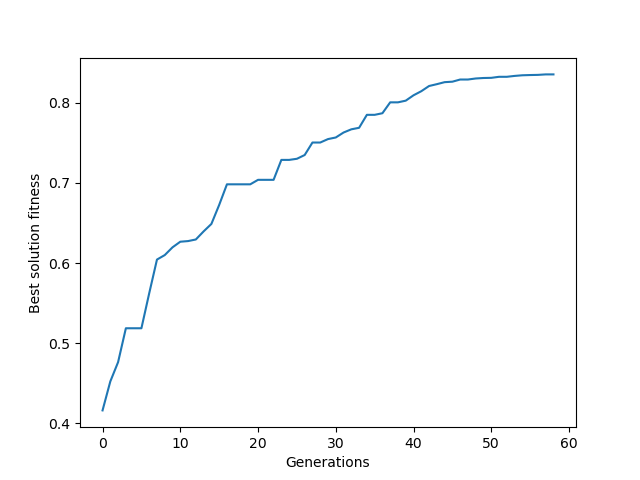
\includegraphics[width=\textwidth]{images/7.png}
                         \caption*{Περίπτωση: 200, 0.6 ,0.01}
                     \end{subfigure}
                     \begin{subfigure}[h]{0.7\textwidth}
                         \centering
                         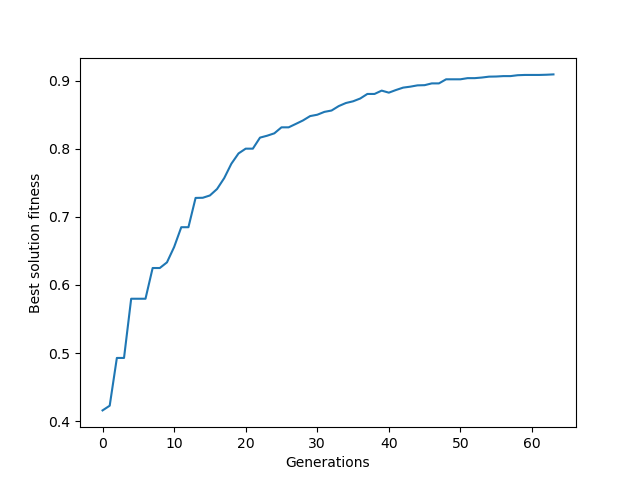
\includegraphics[width=\textwidth]{images/8.png}
                         \caption*{Περίπτωση: 200, 0.6 ,0.10}
                     \end{subfigure}
                     \begin{subfigure}[h]{0.7\textwidth}
                         \centering
                         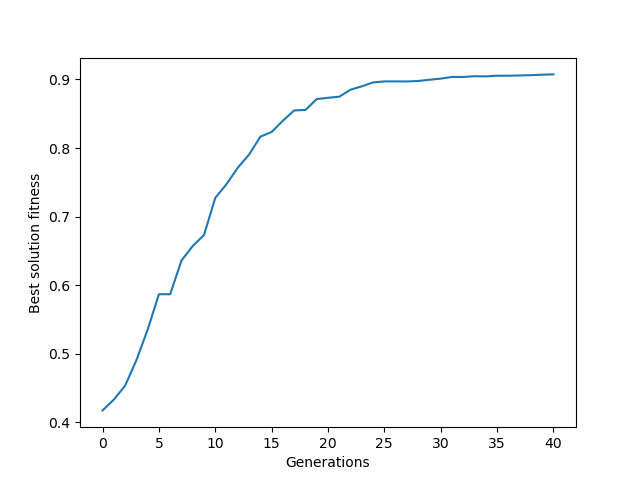
\includegraphics[width=\textwidth]{images/9.png}
                         \caption*{Περίπτωση: 200, 0.9 ,0.01}
                     \end{subfigure}
                 \end{figure}
                 \begin{figure}[H]
                     \centering
                     \begin{subfigure}[ht]{0.7\textwidth}
                         \centering
                         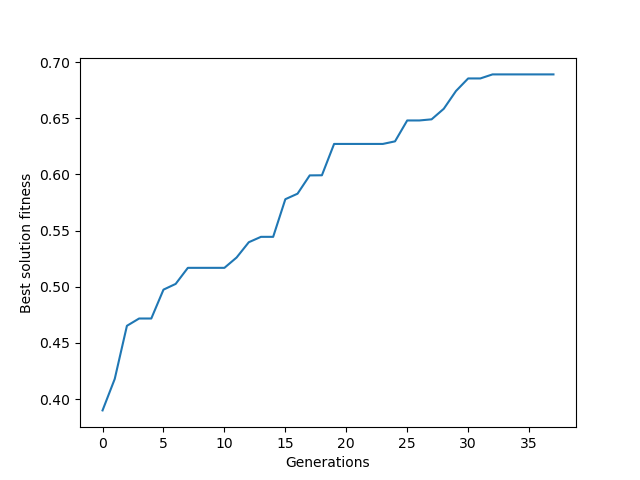
\includegraphics[width=\textwidth]{images/10.png}
                         \caption*{Περίπτωση: 200, 0.1 ,0.01}
                     \end{subfigure}
                \end{figure} 
            \item Συμπεράσματα: 
        \end{enumerate}
\end{document}
